% Created by tikzDevice version 0.10.1 on 2016-12-17 10:47:29
% !TEX encoding = UTF-8 Unicode
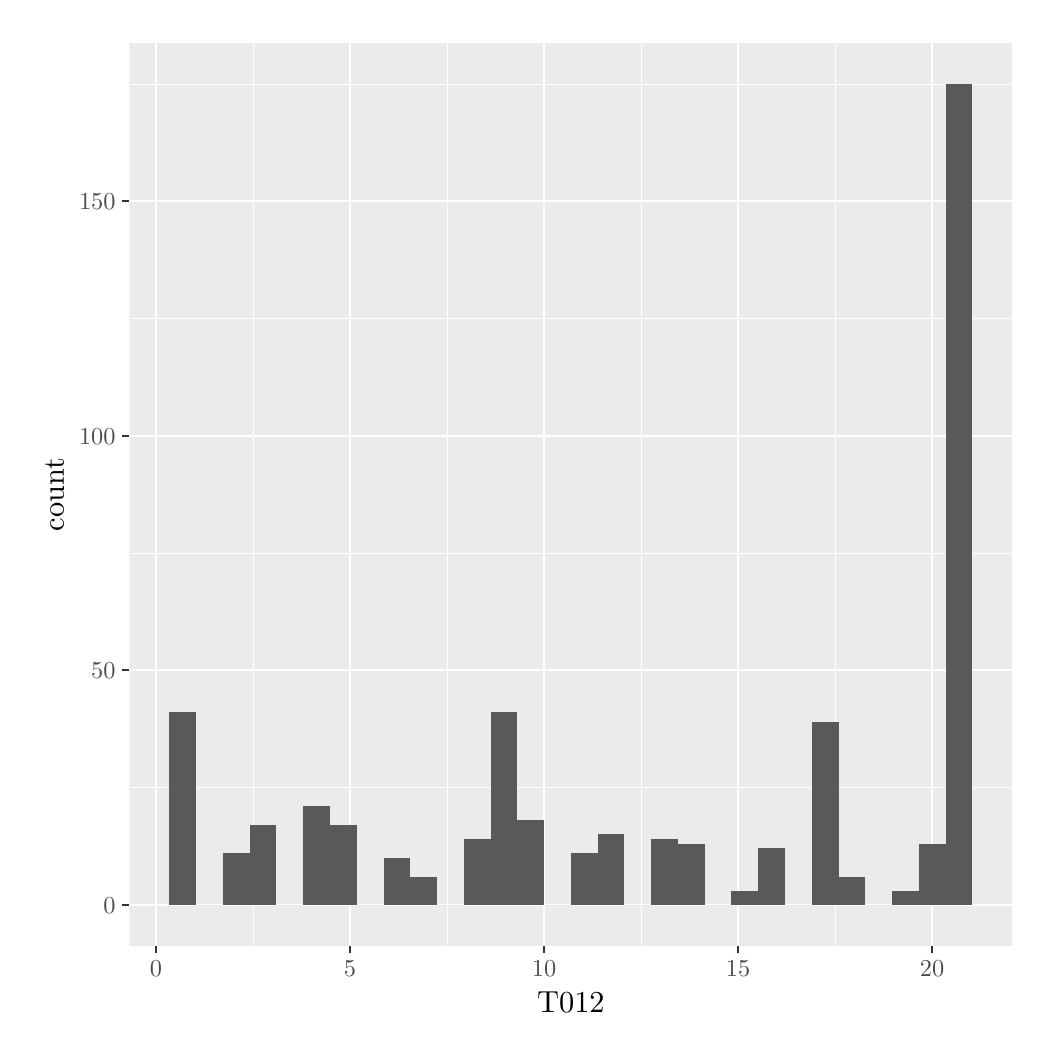
\begin{tikzpicture}[x=1pt,y=1pt]
\definecolor{fillColor}{RGB}{255,255,255}
\path[use as bounding box,fill=fillColor,fill opacity=0.00] (0,0) rectangle (361.35,361.35);
\begin{scope}
\path[clip] (  0.00,  0.00) rectangle (361.35,361.35);
\definecolor{drawColor}{RGB}{255,255,255}
\definecolor{fillColor}{RGB}{255,255,255}

\path[draw=drawColor,line width= 0.6pt,line join=round,line cap=round,fill=fillColor] (  0.00, -0.00) rectangle (361.35,361.35);
\end{scope}
\begin{scope}
\path[clip] ( 36.72, 29.59) rectangle (355.85,355.85);
\definecolor{fillColor}{gray}{0.92}

\path[fill=fillColor] ( 36.72, 29.59) rectangle (355.85,355.85);
\definecolor{drawColor}{RGB}{255,255,255}

\path[draw=drawColor,line width= 0.3pt,line join=round] ( 36.72, 86.79) --
	(355.85, 86.79);

\path[draw=drawColor,line width= 0.3pt,line join=round] ( 36.72,171.53) --
	(355.85,171.53);

\path[draw=drawColor,line width= 0.3pt,line join=round] ( 36.72,256.28) --
	(355.85,256.28);

\path[draw=drawColor,line width= 0.3pt,line join=round] ( 36.72,341.02) --
	(355.85,341.02);

\path[draw=drawColor,line width= 0.3pt,line join=round] ( 81.45, 29.59) --
	( 81.45,355.85);

\path[draw=drawColor,line width= 0.3pt,line join=round] (151.56, 29.59) --
	(151.56,355.85);

\path[draw=drawColor,line width= 0.3pt,line join=round] (221.67, 29.59) --
	(221.67,355.85);

\path[draw=drawColor,line width= 0.3pt,line join=round] (291.78, 29.59) --
	(291.78,355.85);

\path[draw=drawColor,line width= 0.6pt,line join=round] ( 36.72, 44.42) --
	(355.85, 44.42);

\path[draw=drawColor,line width= 0.6pt,line join=round] ( 36.72,129.16) --
	(355.85,129.16);

\path[draw=drawColor,line width= 0.6pt,line join=round] ( 36.72,213.90) --
	(355.85,213.90);

\path[draw=drawColor,line width= 0.6pt,line join=round] ( 36.72,298.65) --
	(355.85,298.65);

\path[draw=drawColor,line width= 0.6pt,line join=round] ( 46.39, 29.59) --
	( 46.39,355.85);

\path[draw=drawColor,line width= 0.6pt,line join=round] (116.50, 29.59) --
	(116.50,355.85);

\path[draw=drawColor,line width= 0.6pt,line join=round] (186.62, 29.59) --
	(186.62,355.85);

\path[draw=drawColor,line width= 0.6pt,line join=round] (256.73, 29.59) --
	(256.73,355.85);

\path[draw=drawColor,line width= 0.6pt,line join=round] (326.84, 29.59) --
	(326.84,355.85);
\definecolor{fillColor}{gray}{0.35}

\path[fill=fillColor] ( 51.23, 44.42) rectangle ( 60.90,113.91);

\path[fill=fillColor] ( 60.90, 44.42) rectangle ( 70.57, 44.42);

\path[fill=fillColor] ( 70.57, 44.42) rectangle ( 80.24, 63.06);

\path[fill=fillColor] ( 80.24, 44.42) rectangle ( 89.91, 73.23);

\path[fill=fillColor] ( 89.91, 44.42) rectangle ( 99.58, 44.42);

\path[fill=fillColor] ( 99.58, 44.42) rectangle (109.25, 80.01);

\path[fill=fillColor] (109.25, 44.42) rectangle (118.92, 73.23);

\path[fill=fillColor] (118.92, 44.42) rectangle (128.59, 44.42);

\path[fill=fillColor] (128.59, 44.42) rectangle (138.26, 61.37);

\path[fill=fillColor] (138.26, 44.42) rectangle (147.93, 54.59);

\path[fill=fillColor] (147.93, 44.42) rectangle (157.60, 44.42);

\path[fill=fillColor] (157.60, 44.42) rectangle (167.27, 68.15);

\path[fill=fillColor] (167.27, 44.42) rectangle (176.95,113.91);

\path[fill=fillColor] (176.95, 44.42) rectangle (186.62, 74.92);

\path[fill=fillColor] (186.62, 44.42) rectangle (196.29, 44.42);

\path[fill=fillColor] (196.29, 44.42) rectangle (205.96, 63.06);

\path[fill=fillColor] (205.96, 44.42) rectangle (215.63, 69.84);

\path[fill=fillColor] (215.63, 44.42) rectangle (225.30, 44.42);

\path[fill=fillColor] (225.30, 44.42) rectangle (234.97, 68.15);

\path[fill=fillColor] (234.97, 44.42) rectangle (244.64, 66.45);

\path[fill=fillColor] (244.64, 44.42) rectangle (254.31, 44.42);

\path[fill=fillColor] (254.31, 44.42) rectangle (263.98, 49.50);

\path[fill=fillColor] (263.98, 44.42) rectangle (273.65, 64.76);

\path[fill=fillColor] (273.65, 44.42) rectangle (283.32, 44.42);

\path[fill=fillColor] (283.32, 44.42) rectangle (292.99,110.52);

\path[fill=fillColor] (292.99, 44.42) rectangle (302.66, 54.59);

\path[fill=fillColor] (302.66, 44.42) rectangle (312.33, 44.42);

\path[fill=fillColor] (312.33, 44.42) rectangle (322.00, 49.50);

\path[fill=fillColor] (322.00, 44.42) rectangle (331.67, 66.45);

\path[fill=fillColor] (331.67, 44.42) rectangle (341.34,341.02);
\end{scope}
\begin{scope}
\path[clip] (  0.00,  0.00) rectangle (361.35,361.35);
\definecolor{drawColor}{gray}{0.30}

\node[text=drawColor,anchor=base east,inner sep=0pt, outer sep=0pt, scale=  0.88] at ( 31.77, 41.39) {0};

\node[text=drawColor,anchor=base east,inner sep=0pt, outer sep=0pt, scale=  0.88] at ( 31.77,126.13) {50};

\node[text=drawColor,anchor=base east,inner sep=0pt, outer sep=0pt, scale=  0.88] at ( 31.77,210.87) {100};

\node[text=drawColor,anchor=base east,inner sep=0pt, outer sep=0pt, scale=  0.88] at ( 31.77,295.62) {150};
\end{scope}
\begin{scope}
\path[clip] (  0.00,  0.00) rectangle (361.35,361.35);
\definecolor{drawColor}{gray}{0.20}

\path[draw=drawColor,line width= 0.6pt,line join=round] ( 33.97, 44.42) --
	( 36.72, 44.42);

\path[draw=drawColor,line width= 0.6pt,line join=round] ( 33.97,129.16) --
	( 36.72,129.16);

\path[draw=drawColor,line width= 0.6pt,line join=round] ( 33.97,213.90) --
	( 36.72,213.90);

\path[draw=drawColor,line width= 0.6pt,line join=round] ( 33.97,298.65) --
	( 36.72,298.65);
\end{scope}
\begin{scope}
\path[clip] (  0.00,  0.00) rectangle (361.35,361.35);
\definecolor{drawColor}{gray}{0.20}

\path[draw=drawColor,line width= 0.6pt,line join=round] ( 46.39, 26.84) --
	( 46.39, 29.59);

\path[draw=drawColor,line width= 0.6pt,line join=round] (116.50, 26.84) --
	(116.50, 29.59);

\path[draw=drawColor,line width= 0.6pt,line join=round] (186.62, 26.84) --
	(186.62, 29.59);

\path[draw=drawColor,line width= 0.6pt,line join=round] (256.73, 26.84) --
	(256.73, 29.59);

\path[draw=drawColor,line width= 0.6pt,line join=round] (326.84, 26.84) --
	(326.84, 29.59);
\end{scope}
\begin{scope}
\path[clip] (  0.00,  0.00) rectangle (361.35,361.35);
\definecolor{drawColor}{gray}{0.30}

\node[text=drawColor,anchor=base,inner sep=0pt, outer sep=0pt, scale=  0.88] at ( 46.39, 18.58) {0};

\node[text=drawColor,anchor=base,inner sep=0pt, outer sep=0pt, scale=  0.88] at (116.50, 18.58) {5};

\node[text=drawColor,anchor=base,inner sep=0pt, outer sep=0pt, scale=  0.88] at (186.62, 18.58) {10};

\node[text=drawColor,anchor=base,inner sep=0pt, outer sep=0pt, scale=  0.88] at (256.73, 18.58) {15};

\node[text=drawColor,anchor=base,inner sep=0pt, outer sep=0pt, scale=  0.88] at (326.84, 18.58) {20};
\end{scope}
\begin{scope}
\path[clip] (  0.00,  0.00) rectangle (361.35,361.35);
\definecolor{drawColor}{RGB}{0,0,0}

\node[text=drawColor,anchor=base,inner sep=0pt, outer sep=0pt, scale=  1.10] at (196.29,  5.50) {T012};
\end{scope}
\begin{scope}
\path[clip] (  0.00,  0.00) rectangle (361.35,361.35);
\definecolor{drawColor}{RGB}{0,0,0}

\node[text=drawColor,rotate= 90.00,anchor=base,inner sep=0pt, outer sep=0pt, scale=  1.10] at ( 13.08,192.72) {count};
\end{scope}
\end{tikzpicture}
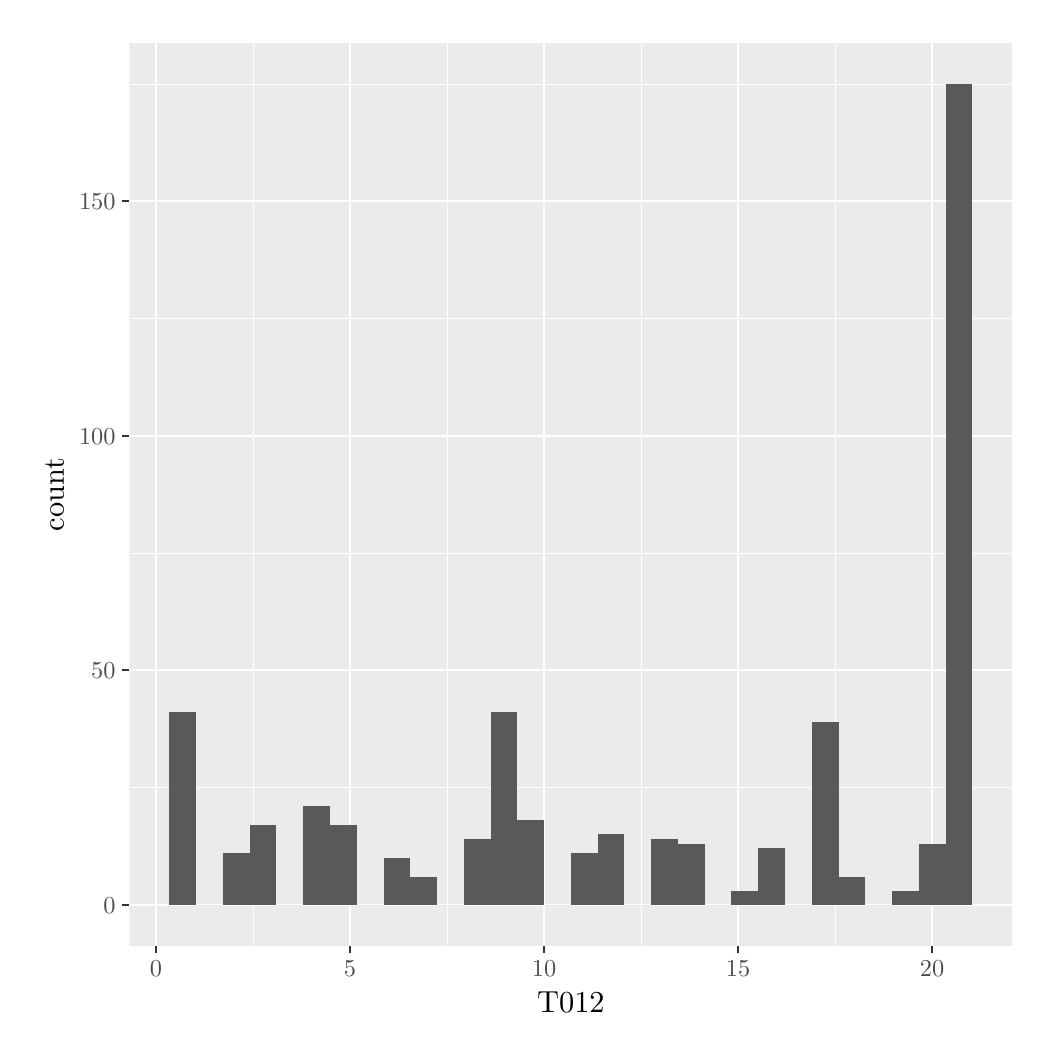
\begin{tikzpicture}[x=1pt,y=1pt]
\definecolor{fillColor}{RGB}{255,255,255}
\path[use as bounding box,fill=fillColor,fill opacity=0.00] (0,0) rectangle (361.35,361.35);
\begin{scope}
\path[clip] (  0.00,  0.00) rectangle (361.35,361.35);
\definecolor{drawColor}{RGB}{255,255,255}
\definecolor{fillColor}{RGB}{255,255,255}

\path[draw=drawColor,line width= 0.6pt,line join=round,line cap=round,fill=fillColor] (  0.00, -0.00) rectangle (361.35,361.35);
\end{scope}
\begin{scope}
\path[clip] ( 36.72, 29.59) rectangle (355.85,355.85);
\definecolor{fillColor}{gray}{0.92}

\path[fill=fillColor] ( 36.72, 29.59) rectangle (355.85,355.85);
\definecolor{drawColor}{RGB}{255,255,255}

\path[draw=drawColor,line width= 0.3pt,line join=round] ( 36.72, 86.79) --
	(355.85, 86.79);

\path[draw=drawColor,line width= 0.3pt,line join=round] ( 36.72,171.53) --
	(355.85,171.53);

\path[draw=drawColor,line width= 0.3pt,line join=round] ( 36.72,256.28) --
	(355.85,256.28);

\path[draw=drawColor,line width= 0.3pt,line join=round] ( 36.72,341.02) --
	(355.85,341.02);

\path[draw=drawColor,line width= 0.3pt,line join=round] ( 81.45, 29.59) --
	( 81.45,355.85);

\path[draw=drawColor,line width= 0.3pt,line join=round] (151.56, 29.59) --
	(151.56,355.85);

\path[draw=drawColor,line width= 0.3pt,line join=round] (221.67, 29.59) --
	(221.67,355.85);

\path[draw=drawColor,line width= 0.3pt,line join=round] (291.78, 29.59) --
	(291.78,355.85);

\path[draw=drawColor,line width= 0.6pt,line join=round] ( 36.72, 44.42) --
	(355.85, 44.42);

\path[draw=drawColor,line width= 0.6pt,line join=round] ( 36.72,129.16) --
	(355.85,129.16);

\path[draw=drawColor,line width= 0.6pt,line join=round] ( 36.72,213.90) --
	(355.85,213.90);

\path[draw=drawColor,line width= 0.6pt,line join=round] ( 36.72,298.65) --
	(355.85,298.65);

\path[draw=drawColor,line width= 0.6pt,line join=round] ( 46.39, 29.59) --
	( 46.39,355.85);

\path[draw=drawColor,line width= 0.6pt,line join=round] (116.50, 29.59) --
	(116.50,355.85);

\path[draw=drawColor,line width= 0.6pt,line join=round] (186.62, 29.59) --
	(186.62,355.85);

\path[draw=drawColor,line width= 0.6pt,line join=round] (256.73, 29.59) --
	(256.73,355.85);

\path[draw=drawColor,line width= 0.6pt,line join=round] (326.84, 29.59) --
	(326.84,355.85);
\definecolor{fillColor}{gray}{0.35}

\path[fill=fillColor] ( 51.23, 44.42) rectangle ( 60.90,113.91);

\path[fill=fillColor] ( 60.90, 44.42) rectangle ( 70.57, 44.42);

\path[fill=fillColor] ( 70.57, 44.42) rectangle ( 80.24, 63.06);

\path[fill=fillColor] ( 80.24, 44.42) rectangle ( 89.91, 73.23);

\path[fill=fillColor] ( 89.91, 44.42) rectangle ( 99.58, 44.42);

\path[fill=fillColor] ( 99.58, 44.42) rectangle (109.25, 80.01);

\path[fill=fillColor] (109.25, 44.42) rectangle (118.92, 73.23);

\path[fill=fillColor] (118.92, 44.42) rectangle (128.59, 44.42);

\path[fill=fillColor] (128.59, 44.42) rectangle (138.26, 61.37);

\path[fill=fillColor] (138.26, 44.42) rectangle (147.93, 54.59);

\path[fill=fillColor] (147.93, 44.42) rectangle (157.60, 44.42);

\path[fill=fillColor] (157.60, 44.42) rectangle (167.27, 68.15);

\path[fill=fillColor] (167.27, 44.42) rectangle (176.95,113.91);

\path[fill=fillColor] (176.95, 44.42) rectangle (186.62, 74.92);

\path[fill=fillColor] (186.62, 44.42) rectangle (196.29, 44.42);

\path[fill=fillColor] (196.29, 44.42) rectangle (205.96, 63.06);

\path[fill=fillColor] (205.96, 44.42) rectangle (215.63, 69.84);

\path[fill=fillColor] (215.63, 44.42) rectangle (225.30, 44.42);

\path[fill=fillColor] (225.30, 44.42) rectangle (234.97, 68.15);

\path[fill=fillColor] (234.97, 44.42) rectangle (244.64, 66.45);

\path[fill=fillColor] (244.64, 44.42) rectangle (254.31, 44.42);

\path[fill=fillColor] (254.31, 44.42) rectangle (263.98, 49.50);

\path[fill=fillColor] (263.98, 44.42) rectangle (273.65, 64.76);

\path[fill=fillColor] (273.65, 44.42) rectangle (283.32, 44.42);

\path[fill=fillColor] (283.32, 44.42) rectangle (292.99,110.52);

\path[fill=fillColor] (292.99, 44.42) rectangle (302.66, 54.59);

\path[fill=fillColor] (302.66, 44.42) rectangle (312.33, 44.42);

\path[fill=fillColor] (312.33, 44.42) rectangle (322.00, 49.50);

\path[fill=fillColor] (322.00, 44.42) rectangle (331.67, 66.45);

\path[fill=fillColor] (331.67, 44.42) rectangle (341.34,341.02);
\end{scope}
\begin{scope}
\path[clip] (  0.00,  0.00) rectangle (361.35,361.35);
\definecolor{drawColor}{gray}{0.30}

\node[text=drawColor,anchor=base east,inner sep=0pt, outer sep=0pt, scale=  0.88] at ( 31.77, 41.39) {0};

\node[text=drawColor,anchor=base east,inner sep=0pt, outer sep=0pt, scale=  0.88] at ( 31.77,126.13) {50};

\node[text=drawColor,anchor=base east,inner sep=0pt, outer sep=0pt, scale=  0.88] at ( 31.77,210.87) {100};

\node[text=drawColor,anchor=base east,inner sep=0pt, outer sep=0pt, scale=  0.88] at ( 31.77,295.62) {150};
\end{scope}
\begin{scope}
\path[clip] (  0.00,  0.00) rectangle (361.35,361.35);
\definecolor{drawColor}{gray}{0.20}

\path[draw=drawColor,line width= 0.6pt,line join=round] ( 33.97, 44.42) --
	( 36.72, 44.42);

\path[draw=drawColor,line width= 0.6pt,line join=round] ( 33.97,129.16) --
	( 36.72,129.16);

\path[draw=drawColor,line width= 0.6pt,line join=round] ( 33.97,213.90) --
	( 36.72,213.90);

\path[draw=drawColor,line width= 0.6pt,line join=round] ( 33.97,298.65) --
	( 36.72,298.65);
\end{scope}
\begin{scope}
\path[clip] (  0.00,  0.00) rectangle (361.35,361.35);
\definecolor{drawColor}{gray}{0.20}

\path[draw=drawColor,line width= 0.6pt,line join=round] ( 46.39, 26.84) --
	( 46.39, 29.59);

\path[draw=drawColor,line width= 0.6pt,line join=round] (116.50, 26.84) --
	(116.50, 29.59);

\path[draw=drawColor,line width= 0.6pt,line join=round] (186.62, 26.84) --
	(186.62, 29.59);

\path[draw=drawColor,line width= 0.6pt,line join=round] (256.73, 26.84) --
	(256.73, 29.59);

\path[draw=drawColor,line width= 0.6pt,line join=round] (326.84, 26.84) --
	(326.84, 29.59);
\end{scope}
\begin{scope}
\path[clip] (  0.00,  0.00) rectangle (361.35,361.35);
\definecolor{drawColor}{gray}{0.30}

\node[text=drawColor,anchor=base,inner sep=0pt, outer sep=0pt, scale=  0.88] at ( 46.39, 18.58) {0};

\node[text=drawColor,anchor=base,inner sep=0pt, outer sep=0pt, scale=  0.88] at (116.50, 18.58) {5};

\node[text=drawColor,anchor=base,inner sep=0pt, outer sep=0pt, scale=  0.88] at (186.62, 18.58) {10};

\node[text=drawColor,anchor=base,inner sep=0pt, outer sep=0pt, scale=  0.88] at (256.73, 18.58) {15};

\node[text=drawColor,anchor=base,inner sep=0pt, outer sep=0pt, scale=  0.88] at (326.84, 18.58) {20};
\end{scope}
\begin{scope}
\path[clip] (  0.00,  0.00) rectangle (361.35,361.35);
\definecolor{drawColor}{RGB}{0,0,0}

\node[text=drawColor,anchor=base,inner sep=0pt, outer sep=0pt, scale=  1.10] at (196.29,  5.50) {T012};
\end{scope}
\begin{scope}
\path[clip] (  0.00,  0.00) rectangle (361.35,361.35);
\definecolor{drawColor}{RGB}{0,0,0}

\node[text=drawColor,rotate= 90.00,anchor=base,inner sep=0pt, outer sep=0pt, scale=  1.10] at ( 13.08,192.72) {count};
\end{scope}
\end{tikzpicture}
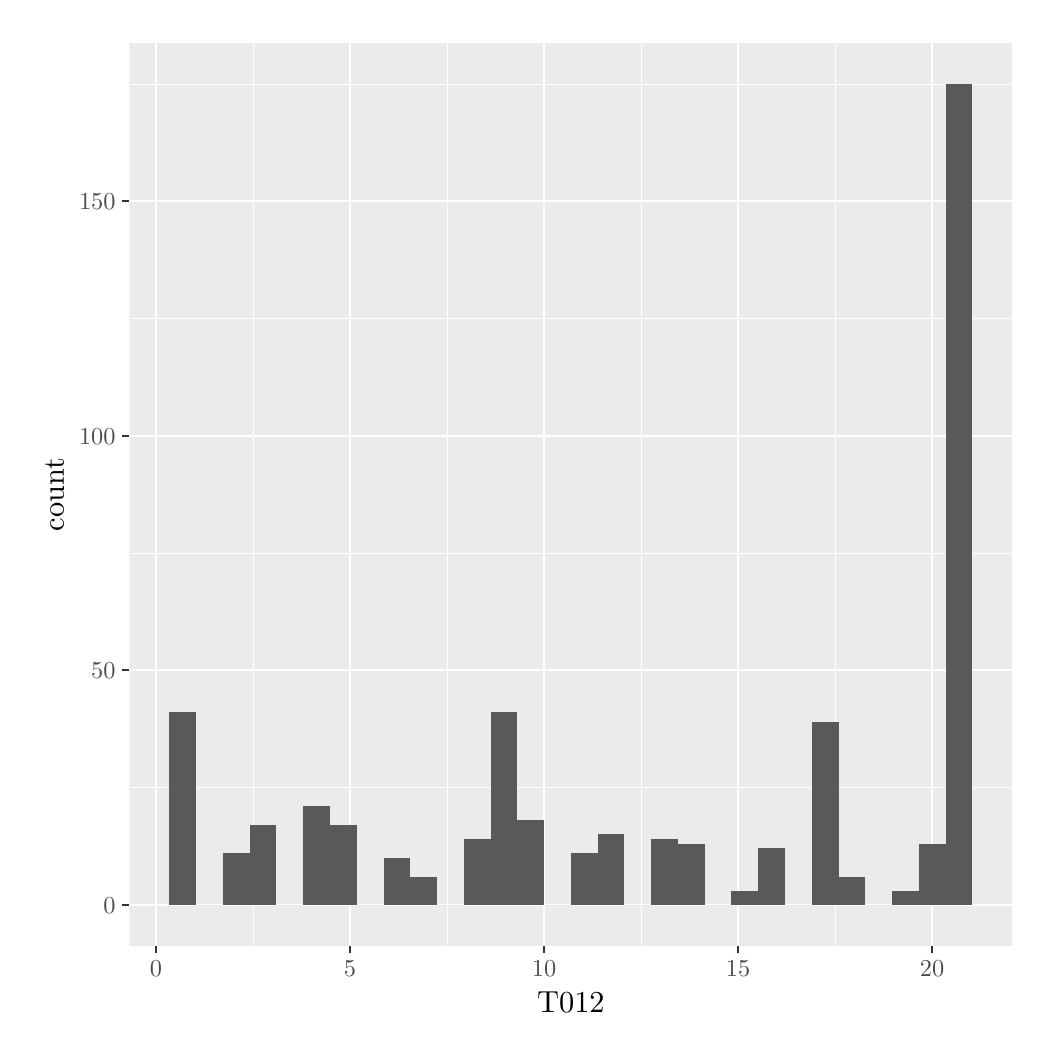
\begin{tikzpicture}[x=1pt,y=1pt]
\definecolor{fillColor}{RGB}{255,255,255}
\path[use as bounding box,fill=fillColor,fill opacity=0.00] (0,0) rectangle (361.35,361.35);
\begin{scope}
\path[clip] (  0.00,  0.00) rectangle (361.35,361.35);
\definecolor{drawColor}{RGB}{255,255,255}
\definecolor{fillColor}{RGB}{255,255,255}

\path[draw=drawColor,line width= 0.6pt,line join=round,line cap=round,fill=fillColor] (  0.00, -0.00) rectangle (361.35,361.35);
\end{scope}
\begin{scope}
\path[clip] ( 36.72, 29.59) rectangle (355.85,355.85);
\definecolor{fillColor}{gray}{0.92}

\path[fill=fillColor] ( 36.72, 29.59) rectangle (355.85,355.85);
\definecolor{drawColor}{RGB}{255,255,255}

\path[draw=drawColor,line width= 0.3pt,line join=round] ( 36.72, 86.79) --
	(355.85, 86.79);

\path[draw=drawColor,line width= 0.3pt,line join=round] ( 36.72,171.53) --
	(355.85,171.53);

\path[draw=drawColor,line width= 0.3pt,line join=round] ( 36.72,256.28) --
	(355.85,256.28);

\path[draw=drawColor,line width= 0.3pt,line join=round] ( 36.72,341.02) --
	(355.85,341.02);

\path[draw=drawColor,line width= 0.3pt,line join=round] ( 81.45, 29.59) --
	( 81.45,355.85);

\path[draw=drawColor,line width= 0.3pt,line join=round] (151.56, 29.59) --
	(151.56,355.85);

\path[draw=drawColor,line width= 0.3pt,line join=round] (221.67, 29.59) --
	(221.67,355.85);

\path[draw=drawColor,line width= 0.3pt,line join=round] (291.78, 29.59) --
	(291.78,355.85);

\path[draw=drawColor,line width= 0.6pt,line join=round] ( 36.72, 44.42) --
	(355.85, 44.42);

\path[draw=drawColor,line width= 0.6pt,line join=round] ( 36.72,129.16) --
	(355.85,129.16);

\path[draw=drawColor,line width= 0.6pt,line join=round] ( 36.72,213.90) --
	(355.85,213.90);

\path[draw=drawColor,line width= 0.6pt,line join=round] ( 36.72,298.65) --
	(355.85,298.65);

\path[draw=drawColor,line width= 0.6pt,line join=round] ( 46.39, 29.59) --
	( 46.39,355.85);

\path[draw=drawColor,line width= 0.6pt,line join=round] (116.50, 29.59) --
	(116.50,355.85);

\path[draw=drawColor,line width= 0.6pt,line join=round] (186.62, 29.59) --
	(186.62,355.85);

\path[draw=drawColor,line width= 0.6pt,line join=round] (256.73, 29.59) --
	(256.73,355.85);

\path[draw=drawColor,line width= 0.6pt,line join=round] (326.84, 29.59) --
	(326.84,355.85);
\definecolor{fillColor}{gray}{0.35}

\path[fill=fillColor] ( 51.23, 44.42) rectangle ( 60.90,113.91);

\path[fill=fillColor] ( 60.90, 44.42) rectangle ( 70.57, 44.42);

\path[fill=fillColor] ( 70.57, 44.42) rectangle ( 80.24, 63.06);

\path[fill=fillColor] ( 80.24, 44.42) rectangle ( 89.91, 73.23);

\path[fill=fillColor] ( 89.91, 44.42) rectangle ( 99.58, 44.42);

\path[fill=fillColor] ( 99.58, 44.42) rectangle (109.25, 80.01);

\path[fill=fillColor] (109.25, 44.42) rectangle (118.92, 73.23);

\path[fill=fillColor] (118.92, 44.42) rectangle (128.59, 44.42);

\path[fill=fillColor] (128.59, 44.42) rectangle (138.26, 61.37);

\path[fill=fillColor] (138.26, 44.42) rectangle (147.93, 54.59);

\path[fill=fillColor] (147.93, 44.42) rectangle (157.60, 44.42);

\path[fill=fillColor] (157.60, 44.42) rectangle (167.27, 68.15);

\path[fill=fillColor] (167.27, 44.42) rectangle (176.95,113.91);

\path[fill=fillColor] (176.95, 44.42) rectangle (186.62, 74.92);

\path[fill=fillColor] (186.62, 44.42) rectangle (196.29, 44.42);

\path[fill=fillColor] (196.29, 44.42) rectangle (205.96, 63.06);

\path[fill=fillColor] (205.96, 44.42) rectangle (215.63, 69.84);

\path[fill=fillColor] (215.63, 44.42) rectangle (225.30, 44.42);

\path[fill=fillColor] (225.30, 44.42) rectangle (234.97, 68.15);

\path[fill=fillColor] (234.97, 44.42) rectangle (244.64, 66.45);

\path[fill=fillColor] (244.64, 44.42) rectangle (254.31, 44.42);

\path[fill=fillColor] (254.31, 44.42) rectangle (263.98, 49.50);

\path[fill=fillColor] (263.98, 44.42) rectangle (273.65, 64.76);

\path[fill=fillColor] (273.65, 44.42) rectangle (283.32, 44.42);

\path[fill=fillColor] (283.32, 44.42) rectangle (292.99,110.52);

\path[fill=fillColor] (292.99, 44.42) rectangle (302.66, 54.59);

\path[fill=fillColor] (302.66, 44.42) rectangle (312.33, 44.42);

\path[fill=fillColor] (312.33, 44.42) rectangle (322.00, 49.50);

\path[fill=fillColor] (322.00, 44.42) rectangle (331.67, 66.45);

\path[fill=fillColor] (331.67, 44.42) rectangle (341.34,341.02);
\end{scope}
\begin{scope}
\path[clip] (  0.00,  0.00) rectangle (361.35,361.35);
\definecolor{drawColor}{gray}{0.30}

\node[text=drawColor,anchor=base east,inner sep=0pt, outer sep=0pt, scale=  0.88] at ( 31.77, 41.39) {0};

\node[text=drawColor,anchor=base east,inner sep=0pt, outer sep=0pt, scale=  0.88] at ( 31.77,126.13) {50};

\node[text=drawColor,anchor=base east,inner sep=0pt, outer sep=0pt, scale=  0.88] at ( 31.77,210.87) {100};

\node[text=drawColor,anchor=base east,inner sep=0pt, outer sep=0pt, scale=  0.88] at ( 31.77,295.62) {150};
\end{scope}
\begin{scope}
\path[clip] (  0.00,  0.00) rectangle (361.35,361.35);
\definecolor{drawColor}{gray}{0.20}

\path[draw=drawColor,line width= 0.6pt,line join=round] ( 33.97, 44.42) --
	( 36.72, 44.42);

\path[draw=drawColor,line width= 0.6pt,line join=round] ( 33.97,129.16) --
	( 36.72,129.16);

\path[draw=drawColor,line width= 0.6pt,line join=round] ( 33.97,213.90) --
	( 36.72,213.90);

\path[draw=drawColor,line width= 0.6pt,line join=round] ( 33.97,298.65) --
	( 36.72,298.65);
\end{scope}
\begin{scope}
\path[clip] (  0.00,  0.00) rectangle (361.35,361.35);
\definecolor{drawColor}{gray}{0.20}

\path[draw=drawColor,line width= 0.6pt,line join=round] ( 46.39, 26.84) --
	( 46.39, 29.59);

\path[draw=drawColor,line width= 0.6pt,line join=round] (116.50, 26.84) --
	(116.50, 29.59);

\path[draw=drawColor,line width= 0.6pt,line join=round] (186.62, 26.84) --
	(186.62, 29.59);

\path[draw=drawColor,line width= 0.6pt,line join=round] (256.73, 26.84) --
	(256.73, 29.59);

\path[draw=drawColor,line width= 0.6pt,line join=round] (326.84, 26.84) --
	(326.84, 29.59);
\end{scope}
\begin{scope}
\path[clip] (  0.00,  0.00) rectangle (361.35,361.35);
\definecolor{drawColor}{gray}{0.30}

\node[text=drawColor,anchor=base,inner sep=0pt, outer sep=0pt, scale=  0.88] at ( 46.39, 18.58) {0};

\node[text=drawColor,anchor=base,inner sep=0pt, outer sep=0pt, scale=  0.88] at (116.50, 18.58) {5};

\node[text=drawColor,anchor=base,inner sep=0pt, outer sep=0pt, scale=  0.88] at (186.62, 18.58) {10};

\node[text=drawColor,anchor=base,inner sep=0pt, outer sep=0pt, scale=  0.88] at (256.73, 18.58) {15};

\node[text=drawColor,anchor=base,inner sep=0pt, outer sep=0pt, scale=  0.88] at (326.84, 18.58) {20};
\end{scope}
\begin{scope}
\path[clip] (  0.00,  0.00) rectangle (361.35,361.35);
\definecolor{drawColor}{RGB}{0,0,0}

\node[text=drawColor,anchor=base,inner sep=0pt, outer sep=0pt, scale=  1.10] at (196.29,  5.50) {T012};
\end{scope}
\begin{scope}
\path[clip] (  0.00,  0.00) rectangle (361.35,361.35);
\definecolor{drawColor}{RGB}{0,0,0}

\node[text=drawColor,rotate= 90.00,anchor=base,inner sep=0pt, outer sep=0pt, scale=  1.10] at ( 13.08,192.72) {count};
\end{scope}
\end{tikzpicture}
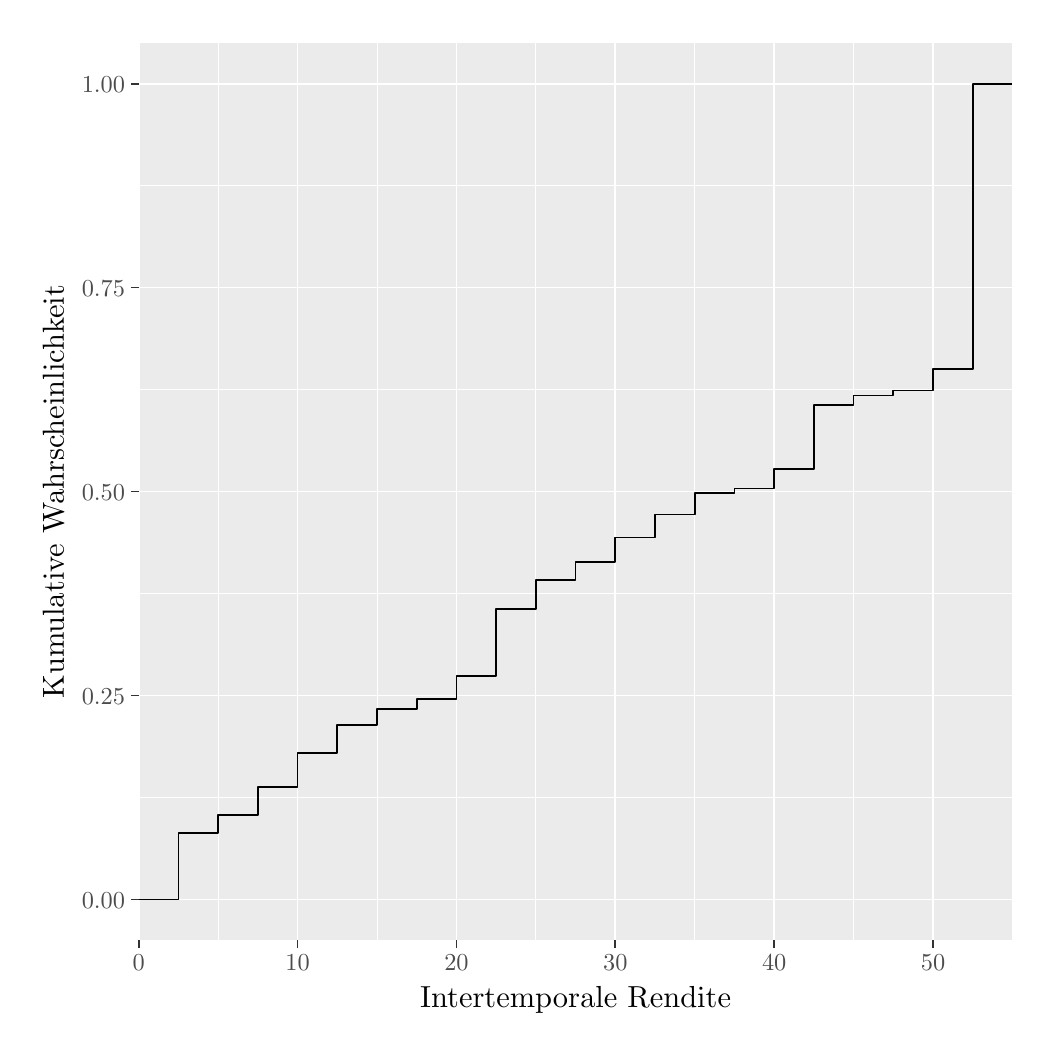
\begin{tikzpicture}[x=1pt,y=1pt]
\definecolor{fillColor}{RGB}{255,255,255}
\path[use as bounding box,fill=fillColor,fill opacity=0.00] (0,0) rectangle (361.35,361.35);
\begin{scope}
\path[clip] (  0.00,  0.00) rectangle (361.35,361.35);
\definecolor{drawColor}{RGB}{255,255,255}
\definecolor{fillColor}{RGB}{255,255,255}

\path[draw=drawColor,line width= 0.6pt,line join=round,line cap=round,fill=fillColor] (  0.00,  0.00) rectangle (361.35,361.35);
\end{scope}
\begin{scope}
\path[clip] ( 40.14, 31.53) rectangle (355.85,355.85);
\definecolor{fillColor}{gray}{0.92}

\path[fill=fillColor] ( 40.14, 31.53) rectangle (355.85,355.85);
\definecolor{drawColor}{RGB}{255,255,255}

\path[draw=drawColor,line width= 0.3pt,line join=round] ( 40.14, 83.13) --
	(355.85, 83.13);

\path[draw=drawColor,line width= 0.3pt,line join=round] ( 40.14,156.84) --
	(355.85,156.84);

\path[draw=drawColor,line width= 0.3pt,line join=round] ( 40.14,230.54) --
	(355.85,230.54);

\path[draw=drawColor,line width= 0.3pt,line join=round] ( 40.14,304.25) --
	(355.85,304.25);

\path[draw=drawColor,line width= 0.3pt,line join=round] ( 68.84, 31.53) --
	( 68.84,355.85);

\path[draw=drawColor,line width= 0.3pt,line join=round] (126.24, 31.53) --
	(126.24,355.85);

\path[draw=drawColor,line width= 0.3pt,line join=round] (183.64, 31.53) --
	(183.64,355.85);

\path[draw=drawColor,line width= 0.3pt,line join=round] (241.05, 31.53) --
	(241.05,355.85);

\path[draw=drawColor,line width= 0.3pt,line join=round] (298.45, 31.53) --
	(298.45,355.85);

\path[draw=drawColor,line width= 0.3pt,line join=round] (355.85, 31.53) --
	(355.85,355.85);

\path[draw=drawColor,line width= 0.6pt,line join=round] ( 40.14, 46.27) --
	(355.85, 46.27);

\path[draw=drawColor,line width= 0.6pt,line join=round] ( 40.14,119.98) --
	(355.85,119.98);

\path[draw=drawColor,line width= 0.6pt,line join=round] ( 40.14,193.69) --
	(355.85,193.69);

\path[draw=drawColor,line width= 0.6pt,line join=round] ( 40.14,267.40) --
	(355.85,267.40);

\path[draw=drawColor,line width= 0.6pt,line join=round] ( 40.14,341.11) --
	(355.85,341.11);

\path[draw=drawColor,line width= 0.6pt,line join=round] ( 40.14, 31.53) --
	( 40.14,355.85);

\path[draw=drawColor,line width= 0.6pt,line join=round] ( 97.54, 31.53) --
	( 97.54,355.85);

\path[draw=drawColor,line width= 0.6pt,line join=round] (154.94, 31.53) --
	(154.94,355.85);

\path[draw=drawColor,line width= 0.6pt,line join=round] (212.34, 31.53) --
	(212.34,355.85);

\path[draw=drawColor,line width= 0.6pt,line join=round] (269.75, 31.53) --
	(269.75,355.85);

\path[draw=drawColor,line width= 0.6pt,line join=round] (327.15, 31.53) --
	(327.15,355.85);
\definecolor{drawColor}{RGB}{0,0,0}

\path[draw=drawColor,line width= 0.6pt,line join=round] ( 40.14, 46.27) --
	( 54.49, 46.27) --
	( 54.49, 70.45) --
	( 68.84, 70.45) --
	( 68.84, 76.94) --
	( 83.19, 76.94) --
	( 83.19, 86.96) --
	( 97.54, 86.96) --
	( 97.54, 99.34) --
	(111.89, 99.34) --
	(111.89,109.37) --
	(126.24,109.37) --
	(126.24,115.26) --
	(140.59,115.26) --
	(140.59,118.80) --
	(154.94,118.80) --
	(154.94,127.06) --
	(169.29,127.06) --
	(169.29,151.23) --
	(183.64,151.23) --
	(183.64,161.85) --
	(197.99,161.85) --
	(197.99,168.33) --
	(212.34,168.33) --
	(212.34,177.18) --
	(226.70,177.18) --
	(226.70,185.43) --
	(241.05,185.43) --
	(241.05,193.10) --
	(255.40,193.10) --
	(255.40,194.87) --
	(269.75,194.87) --
	(269.75,201.95) --
	(284.10,201.95) --
	(284.10,224.94) --
	(298.45,224.94) --
	(298.45,228.48) --
	(312.80,228.48) --
	(312.80,230.25) --
	(327.15,230.25) --
	(327.15,237.92) --
	(341.50,237.92) --
	(341.50,341.11) --
	(355.85,341.11) --
	(355.85,341.11);
\end{scope}
\begin{scope}
\path[clip] (  0.00,  0.00) rectangle (361.35,361.35);
\definecolor{drawColor}{gray}{0.30}

\node[text=drawColor,anchor=base east,inner sep=0pt, outer sep=0pt, scale=  0.88] at ( 35.19, 43.24) {0.00};

\node[text=drawColor,anchor=base east,inner sep=0pt, outer sep=0pt, scale=  0.88] at ( 35.19,116.95) {0.25};

\node[text=drawColor,anchor=base east,inner sep=0pt, outer sep=0pt, scale=  0.88] at ( 35.19,190.66) {0.50};

\node[text=drawColor,anchor=base east,inner sep=0pt, outer sep=0pt, scale=  0.88] at ( 35.19,264.37) {0.75};

\node[text=drawColor,anchor=base east,inner sep=0pt, outer sep=0pt, scale=  0.88] at ( 35.19,338.08) {1.00};
\end{scope}
\begin{scope}
\path[clip] (  0.00,  0.00) rectangle (361.35,361.35);
\definecolor{drawColor}{gray}{0.20}

\path[draw=drawColor,line width= 0.6pt,line join=round] ( 37.39, 46.27) --
	( 40.14, 46.27);

\path[draw=drawColor,line width= 0.6pt,line join=round] ( 37.39,119.98) --
	( 40.14,119.98);

\path[draw=drawColor,line width= 0.6pt,line join=round] ( 37.39,193.69) --
	( 40.14,193.69);

\path[draw=drawColor,line width= 0.6pt,line join=round] ( 37.39,267.40) --
	( 40.14,267.40);

\path[draw=drawColor,line width= 0.6pt,line join=round] ( 37.39,341.11) --
	( 40.14,341.11);
\end{scope}
\begin{scope}
\path[clip] (  0.00,  0.00) rectangle (361.35,361.35);
\definecolor{drawColor}{gray}{0.20}

\path[draw=drawColor,line width= 0.6pt,line join=round] ( 40.14, 28.78) --
	( 40.14, 31.53);

\path[draw=drawColor,line width= 0.6pt,line join=round] ( 97.54, 28.78) --
	( 97.54, 31.53);

\path[draw=drawColor,line width= 0.6pt,line join=round] (154.94, 28.78) --
	(154.94, 31.53);

\path[draw=drawColor,line width= 0.6pt,line join=round] (212.34, 28.78) --
	(212.34, 31.53);

\path[draw=drawColor,line width= 0.6pt,line join=round] (269.75, 28.78) --
	(269.75, 31.53);

\path[draw=drawColor,line width= 0.6pt,line join=round] (327.15, 28.78) --
	(327.15, 31.53);
\end{scope}
\begin{scope}
\path[clip] (  0.00,  0.00) rectangle (361.35,361.35);
\definecolor{drawColor}{gray}{0.30}

\node[text=drawColor,anchor=base,inner sep=0pt, outer sep=0pt, scale=  0.88] at ( 40.14, 20.52) {0};

\node[text=drawColor,anchor=base,inner sep=0pt, outer sep=0pt, scale=  0.88] at ( 97.54, 20.52) {10};

\node[text=drawColor,anchor=base,inner sep=0pt, outer sep=0pt, scale=  0.88] at (154.94, 20.52) {20};

\node[text=drawColor,anchor=base,inner sep=0pt, outer sep=0pt, scale=  0.88] at (212.34, 20.52) {30};

\node[text=drawColor,anchor=base,inner sep=0pt, outer sep=0pt, scale=  0.88] at (269.75, 20.52) {40};

\node[text=drawColor,anchor=base,inner sep=0pt, outer sep=0pt, scale=  0.88] at (327.15, 20.52) {50};
\end{scope}
\begin{scope}
\path[clip] (  0.00,  0.00) rectangle (361.35,361.35);
\definecolor{drawColor}{RGB}{0,0,0}

\node[text=drawColor,anchor=base,inner sep=0pt, outer sep=0pt, scale=  1.10] at (197.99,  7.44) {Intertemporale Rendite};
\end{scope}
\begin{scope}
\path[clip] (  0.00,  0.00) rectangle (361.35,361.35);
\definecolor{drawColor}{RGB}{0,0,0}

\node[text=drawColor,rotate= 90.00,anchor=base,inner sep=0pt, outer sep=0pt, scale=  1.10] at ( 13.08,193.69) {Kumulative Wahrscheinlichkeit};
\end{scope}
\end{tikzpicture}
